\documentclass[10pt, aspectratio=169, handout]{beamer}
\usefonttheme{professionalfonts}

\mode<presentation>{
  \usetheme{Berkeley}
  \usecolortheme{beaver}
  \usefonttheme{default}
  \setbeamertemplate{navigation symbols}{}
  \setbeamertemplate{caption}[numbered]
}

\setbeamertemplate{footline}{%
  \leavevmode%
  \hbox{%
    \begin{beamercolorbox}[wd=.85\paperwidth,ht=2.5ex,dp=1ex,left]{author in head/foot}%
      \usebeamerfont{author in head/foot}Digital Signal Processing, Fall 2025%
    \end{beamercolorbox}%
    \begin{beamercolorbox}[wd=.15\paperwidth,ht=2.5ex,dp=1ex,right]{date in head/foot}%
      \hspace*{0.5em}\insertframenumber{} / \inserttotalframenumber\hspace*{0.5em}%
    \end{beamercolorbox}%
  }%
  \vskip0pt%
}

\usepackage[english]{babel}
\usepackage[utf8]{inputenc}
\usepackage{tikz}
\usepackage{pgfplots}
\usepgfplotslibrary{groupplots}
\usetikzlibrary{calc, positioning, arrows.meta, backgrounds, plotmarks, shapes.geometric}
\pgfplotsset{compat=newest}

\usepackage{array}
\usepackage{makecell}
\usepackage{verbatim}
\usepackage{graphicx}
\usepackage{amsfonts}
\usepackage{amsmath}
\usepackage{bm}
\usepackage{epstopdf}
\usepackage[absolute,overlay]{textpos}
\usepackage{hyperref}
\hypersetup{colorlinks=true, linkcolor=blue, urlcolor=cyan}

\title[DSP]{Discrete Time Filtering}
\author{Maxx Seminario}
\institute{University of Nebraska-Lincoln}
\date{Fall 2025}

\begin{document}

%--------------------------------------------------
\begin{frame}
  \titlepage
\end{frame}

%--------------------------------------------------
\section{Introduction}

\begin{frame}{What is a Filter?}

\textbf{Key Concept:} Filters are LTI systems that modify frequency components of signals.


\textbf{Definition:} Any system that modifies certain frequencies relative to others

\vspace{0.3cm}
\textbf{Two Main Classes:}
\begin{itemize}
  \item \textbf{IIR (Infinite Impulse Response):} Rational transfer function $H(z) = \frac{B(z)}{A(z)}$
  \item \textbf{FIR (Finite Impulse Response):} Polynomial transfer function $H(z) = \sum_{n=0}^{M} b[n]z^{-n}$
\end{itemize}

\vspace{0.3cm}
\textbf{Design Focus:}
\begin{itemize}
  \item Determine parameters to approximate desired frequency response
  \item Meet design specifications
  \item Maintain causality and stability
\end{itemize}

\end{frame}

% %--------------------------------------------------
\section{Classical Filter Types}

% \begin{frame}{Three Classical Approximations}
% \small

% \textbf{Standard continuous-time designs implemented in discrete-time}

% \vspace{0.3cm}
% \textbf{Butterworth:}
% \begin{itemize}
%   \item Monotonic in passband and stopband
%   \item Maximally flat at $\omega = 0$
%   \item All zeros at $z = -1$
% \end{itemize}

% \vspace{0.3cm}
% \textbf{Chebyshev Type I:}
% \begin{itemize}
%   \item Equiripple in passband, monotonic in stopband
%   \item All zeros at $z = -1$
%   \item Lower order than Butterworth for same specs
% \end{itemize}

% \vspace{0.3cm}
% \textbf{Chebyshev Type II:}
% \begin{itemize}
%   \item Monotonic in passband, equiripple in stopband
%   \item Zeros distributed on unit circle in stopband
%   \item Same order as Type I
% \end{itemize}

% \end{frame}

% %--------------------------------------------------
\begin{frame}{Elliptic Filters}
\small

\textbf{Key Concept:} Equiripple in \emph{both} passband and stopband

\vspace{0.3cm}
\textbf{Optimal Property:}
\begin{itemize}
  \item Lowest order filter for given specifications
  \item Minimum approximation error ripples equally in both bands
\end{itemize}

\vspace{0.3cm}
\textbf{Characteristics:}
\begin{itemize}
  \item Zeros arrayed on unit circle in stopband (like Chebyshev II)
  \item Sharpest transition band for given order
\end{itemize}

\vspace{0.3cm}
\textbf{Trade-off:}
\begin{itemize}
  \item Lowest order $\rightarrow$ fewer computations
  \item More complex implementation than Butterworth
  \item Group delay typically less uniform than Butterworth
\end{itemize}

\end{frame}

% %--------------------------------------------------
\section{Design Comparisons}

\begin{frame}{Example Specifications}
\small

\textbf{Common specification for all designs:}

\vspace{0.2cm}
Passband: $0.99 \leq |H(e^{j\omega})| \leq 1. 01$, $|\omega| \leq 0.4\pi$

Stopband: $|H(e^{j\omega})| \leq 0. 001$, $0.6\pi \leq |\omega| \leq \pi$

\vspace{0.3cm}
\begin{center}
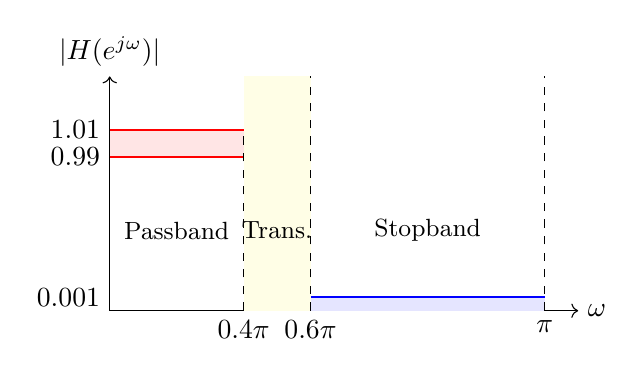
\begin{tikzpicture}[scale=0.85]
  \draw[->] (0,0) -- (7,0) node[right] {$\omega$};
  \draw[->] (0,0) -- (0,3. 5) node[above] {$|H(e^{j\omega})|$};
  
  % Passband
  \fill[red! 10] (0,2. 3) rectangle (2,2.7);
  \draw[thick, red] (0,2.7) -- (2,2.7);
  \draw[thick, red] (0,2.3) -- (2,2.3);
  \draw[dashed] (2,0) -- (2,2.7);
  \node[below] at (2,0) {$0.4\pi$};
  
  % Transition
  \fill[yellow!10] (2,0) rectangle (3,3.5);
  
  % Stopband
  \fill[blue!10] (3,0) rectangle (6. 5,0.2);
  \draw[thick, blue] (3,0. 2) -- (6.5,0.2);
  \draw[dashed] (3,0) -- (3,3.5);
  \node[below] at (3,0) {$0.6\pi$};
  \draw[dashed] (6.5,0) -- (6.5,3.5);
  \node[below] at (6. 5,0) {$\pi$};
  
  % Labels
  \node[left] at (0,2.7) {$1. 01$};
  \node[left] at (0,2.3) {$0.99$};
  \node[left] at (0,0. 2) {$0.001$};
  \node at (1,1.2) {\small Passband};
  \node at (2. 5,1.2) {\small Trans.};
  \node at (4. 75,1.2) {\small Stopband};
\end{tikzpicture}
\end{center}

\end{frame}

% %--------------------------------------------------
\begin{frame}{Filter Order Comparison}
\small

\textbf{For specifications:} $\omega_p = 0.4\pi$, $\omega_s = 0.6\pi$, $\delta_p = 0.01$, $\delta_s = 0.001$

\vspace{0.4cm}
\begin{center}
\begin{tabular}{lcc}
\hline
\textbf{Filter Type} & \textbf{Minimum Order} & \textbf{Zero Locations} \\
\hline
Butterworth & 14 & 14 zeros at $z=-1$ \\
Chebyshev I & 8 & 8 zeros at $z=-1$ \\
Chebyshev II & 8 & 8 zeros on unit circle \\
Elliptic & 6 & 6 zeros on unit circle \\
\hline
\end{tabular}
\end{center}

\vspace{0.4cm}
\textbf{Key Observations:}
\begin{itemize}
  \item Elliptic achieves lowest order (optimal)
  \item Butterworth requires $\sim 2\times$ the order of Chebyshev
  \item Chebyshev I simpler than II (all zeros at $z=-1$)
  \item Order directly impacts computational complexity
\end{itemize}

\end{frame}

%--------------------------------------------------
\section{Butterworth Filter}

\begin{frame}{Butterworth: Magnitude Response}
\small

\textbf{Order 14 Butterworth Filter}

\vspace{0.2cm}
\begin{center}
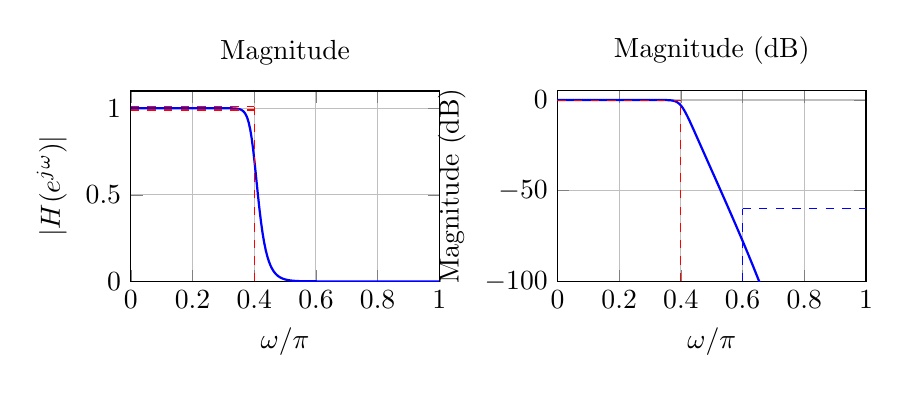
\begin{tikzpicture}
\begin{groupplot}[
    group style={
        group size=2 by 1,
        horizontal sep=1.5cm,
    },
    width=5.5cm,
    height=4cm,
]

% Linear magnitude
\nextgroupplot[
    xlabel={$\omega/\pi$},
    ylabel={$|H(e^{j\omega})|$},
    xmin=0, xmax=1,
    ymin=0, ymax=1. 1,
    grid=major,
    title={Magnitude},
]
\addplot[blue, thick, domain=0:1, samples=200] {1/sqrt(1 + (tan(x*90)/tan(36))^28)};
\draw[red, dashed] (axis cs:0,0.99) -- (axis cs:0. 4,0.99);
\draw[red, dashed] (axis cs:0,1.01) -- (axis cs:0.4,1.01);
\draw[red, dashed] (axis cs:0.4,0) -- (axis cs:0.4,1.01);
\draw[blue, dashed] (axis cs:0.6,0) -- (axis cs:0.6,0.001);
\draw[blue, dashed] (axis cs:0.6,0. 001) -- (axis cs:1,0.001);

% Log magnitude (dB)
\nextgroupplot[
    xlabel={$\omega/\pi$},
    ylabel={Magnitude (dB)},
    xmin=0, xmax=1,
    ymin=-100, ymax=5,
    grid=major,
    title={Magnitude (dB)},
]
\addplot[blue, thick, domain=0:1, samples=200] {20*log10(1/sqrt(1 + (tan(x*90)/tan(36))^28))};
\draw[red, dashed] (axis cs:0,-0.087) -- (axis cs:0. 4,-0.087);
\draw[red, dashed] (axis cs:0. 4,-100) -- (axis cs:0. 4,0);
\draw[blue, dashed] (axis cs:0. 6,-100) -- (axis cs:0. 6,-60);
\draw[blue, dashed] (axis cs:0. 6,-60) -- (axis cs:1,-60);

\end{groupplot}
\end{tikzpicture}
\end{center}

\vspace{0.1cm}
\textbf{Characteristics:}
\begin{itemize}
  \item Smooth, monotonic decrease (no ripple)
  \item Maximally flat at $\omega = 0$
  \item Gradual transition band roll-off
\end{itemize}

\end{frame}

%--------------------------------------------------

\begin{frame}{Butterworth: Pole-Zero Plot (near-vertical poles)}
\small

\textbf{Order 14 Butterworth Filter --- poles near vertical line at small negative Re and bowed left with increasing Im}

\vspace{0.2cm}
\begin{center}
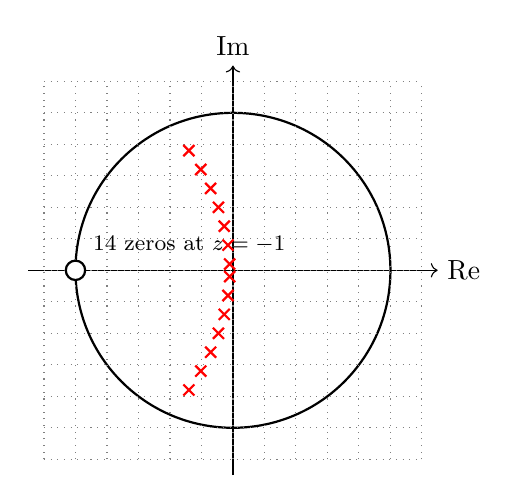
\begin{tikzpicture}[scale=2.0]
  % Unit circle
  \draw[thick] (0,0) circle (1);
  \draw[->] (-1.3,0) -- (1.3,0) node[right] {Re};
  \draw[->] (0,-1.3) -- (0,1.3) node[above] {Im};
  
  % Light grid for reference (optional)
  \draw[gray, dotted] (-1.2,-1.2) grid[step=0.2] (1.2,1.2);
  
  % 14 zeros at z = -1 (represented as a stacked marker with label)
  \node[circle, draw=black, fill=white, thick, minimum size=7pt, inner sep=0pt] at (-1,0) {};
  \node[above right] at (-0.95,0.05) {\footnotesize 14 zeros at $z=-1$};
  
  % Poles: 7 conjugate pairs (N=14)
  % Place poles near a vertical line Re ~= 0 (small negative base), then add a y^2 bow to move them left for larger |Im|.
  % x = -base - bow_coeff * y^2
  \pgfmathsetmacro{\base}{0.02}    % base negative offset from Re=0
  \pgfmathsetmacro{\bow}{0.45}     % bow coefficient (controls how much they lean left)
  \foreach \k in {0,...,6} {
    \pgfmathsetmacro{\y}{0.04 + \k*0.12}               % imag: 0.04, 0.16, ..., up to ~0.76
    % compute x as small negative base plus bow to the left that grows with y^2
    \pgfmathsetmacro{\x}{- \base - \bow * (\y)^2}
    % draw pole as an "X" at (x,y) and its conjugate (x,-y)
    \draw[red, thick] (\x-0.035,\y-0.035) -- (\x+0.035,\y+0.035);
    \draw[red, thick] (\x-0.035,\y+0.035) -- (\x+0.035,\y-0.035);
    \draw[red, thick] (\x-0.035,-\y-0.035) -- (\x+0.035,-\y+0.035);
    \draw[red, thick] (\x-0.035,-\y+0.035) -- (\x+0.035,-\y-0.035);
  }
  
\end{tikzpicture}
\end{center}

\textbf{Key Features:}
\begin{itemize}
  \item Leftward bow increases with $|\mathrm{Im}|$ via a quadratic dependence on Im
  \item All poles kept inside unit circle for stability 
\end{itemize}

\end{frame}

%--------------------------------------------------
\section{Chebyshev Type I Filter}

\begin{frame}{Chebyshev Type I: Magnitude Response}
\small

\textbf{Order 8 Chebyshev Type I Filter}

\vspace{0.2cm}
\begin{center}
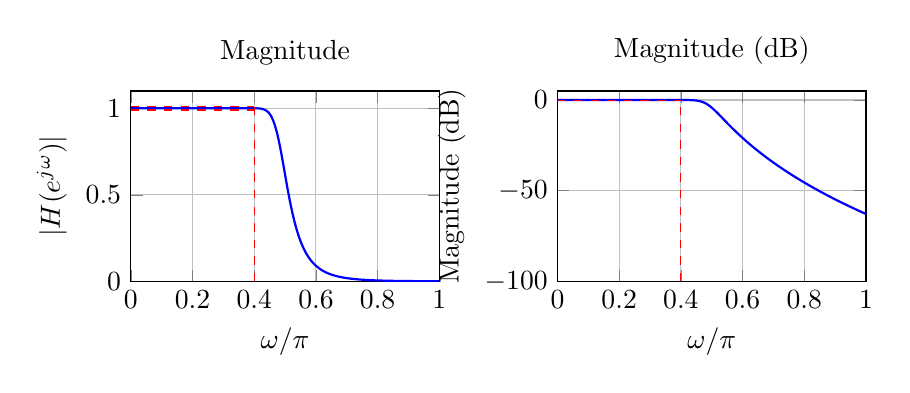
\begin{tikzpicture}
\begin{groupplot}[
    group style={
        group size=2 by 1,
        horizontal sep=1.5cm,
    },
    width=5.5cm,
    height=4cm,
]

% Linear magnitude
\nextgroupplot[
    xlabel={$\omega/\pi$},
    ylabel={$|H(e^{j\omega})|$},
    xmin=0, xmax=1,
    ymin=0, ymax=1.1,
    grid=major,
    title={Magnitude},
]
% Chebyshev Type I approximation with ripple in passband
\addplot[blue, thick, domain=0:0.4, samples=200] {1/(sqrt(1 + 0.01*0.01*(cos(8*acos(x/0.4)))^2))};
\addplot[blue, thick, domain=0.4:1, samples=200] {1/(sqrt(1 + 0.01*0.01*(cosh(8*ln((x/0.4)+sqrt((x/0.4)^2-1))))^2))};
\draw[red, dashed] (axis cs:0,0.99) -- (axis cs:0.4,0.99);
\draw[red, dashed] (axis cs:0,1.01) -- (axis cs:0.4,1.01);
\draw[red, dashed] (axis cs:0.4,0) -- (axis cs:0.4,1.01);

% Log magnitude (dB)
\nextgroupplot[
    xlabel={$\omega/\pi$},
    ylabel={Magnitude (dB)},
    xmin=0, xmax=1,
    ymin=-100, ymax=5,
    grid=major,
    title={Magnitude (dB)},
]
\addplot[blue, thick, domain=0:0.4, samples=200] {20*log10(1/(sqrt(1 + 0.01*0.01*(cos(8*acos(x/0. 4)))^2)))};
\addplot[blue, thick, domain=0.4:1, samples=200] {20*log10(1/(sqrt(1 + 0.01*0.01*(cosh(8*ln((x/0.4)+sqrt((x/0.4)^2-1))))^2)))};
\draw[red, dashed] (axis cs:0,-0.087) -- (axis cs:0. 4,-0.087);
\draw[red, dashed] (axis cs:0.4,-100) -- (axis cs:0. 4,0);

\end{groupplot}
\end{tikzpicture}
\end{center}

\vspace{0.1cm}
\textbf{Characteristics:}
\begin{itemize}
  \item Equiripple in passband (oscillates between 0. 99 and 1.01)
  \item Monotonic in stopband
  \item Sharper transition than Butterworth
\end{itemize}

\end{frame}

%------------------------\begin{frame}{Chebyshev Type I: Pole-Zero Plot (right-half bowed poles)}




\begin{frame}{Chebyshev Type I: Pole-Zero Plot (quadratic bow)}
\small

\begin{columns}[T,onlytextwidth]
  \column{0.58\textwidth}
  \begin{center}
  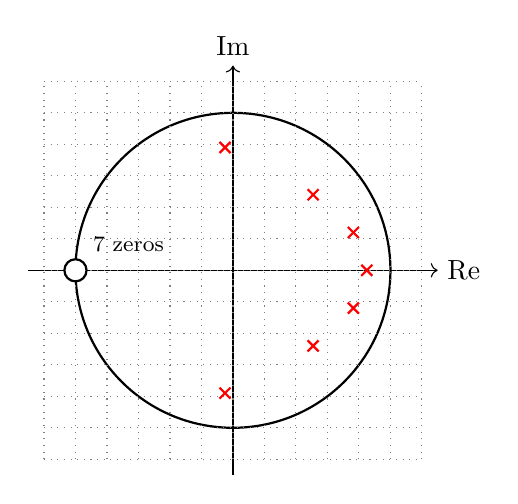
\begin{tikzpicture}[scale=2.0]
    % Parameters for quadratic curve x(y) = a - b y^2
    \pgfmathsetmacro{\a}{0.85}
    \pgfmathsetmacro{\b}{1.48}

    % Unit circle and axes
    \draw[thick] (0,0) circle (1);
    \draw[->] (-1.3,0) -- (1.3,0) node[right] {Re};
    \draw[->] (0,-1.3) -- (0,1.3) node[above] {Im};

    % Grid
    \draw[gray, dotted] (-1.2,-1.2) grid[step=0.2] (1.2,1.2);

    % 7 zeros at z = -1 (stacked visual marker)
    \node[circle, fill=white, draw=black, thick, minimum size=8pt, inner sep=0] at (-1,0) {};
    \node[above right] at (-0.95,0.06) {\footnotesize 7 zeros};

    % Real-axis pole (largest real component)
    \pgfmathsetmacro{\xreal}{\a} % = 0.85
    \draw[red, thick] (\xreal-0.035,-0.035) -- (\xreal+0.035,0.035);
    \draw[red, thick] (\xreal-0.035,0.035) -- (\xreal+0.035,-0.035);

    % Conjugate pairs
    \foreach \y in {0.24,0.48,0.78} {
      \pgfmathsetmacro{\xpole}{\a - \b*(\y*\y)}
      % Pole at (xpole, y)
      \draw[red, thick] (\xpole-0.035,\y-0.035) -- (\xpole+0.035,\y+0.035);
      \draw[red, thick] (\xpole-0.035,\y+0.035) -- (\xpole+0.035,\y-0.035);
      % Conjugate at (xpole, -y)
      \draw[red, thick] (\xpole-0.035,-\y-0.035) -- (\xpole+0.035,-\y+0.035);
      \draw[red, thick] (\xpole-0.035,-\y+0.035) -- (\xpole+0.035,-\y-0.035);
    }
  \end{tikzpicture}
  \end{center}

  \column{0.42\textwidth}
  \textbf{Key Features:}
  \begin{itemize}
    \item 7 zeros stacked at $z=-1$
    \item 7 poles lie on a smooth quadratic curve
    \item All poles remain inside the unit circle
  \end{itemize}
\end{columns}

\end{frame}







%--------------------------------------------------
\section{Chebyshev Type II Filter}

\begin{frame}{Chebyshev Type II: Magnitude Response}
\small

\textbf{Order 8 Chebyshev Type II Filter}

\vspace{0.2cm}
\begin{center}
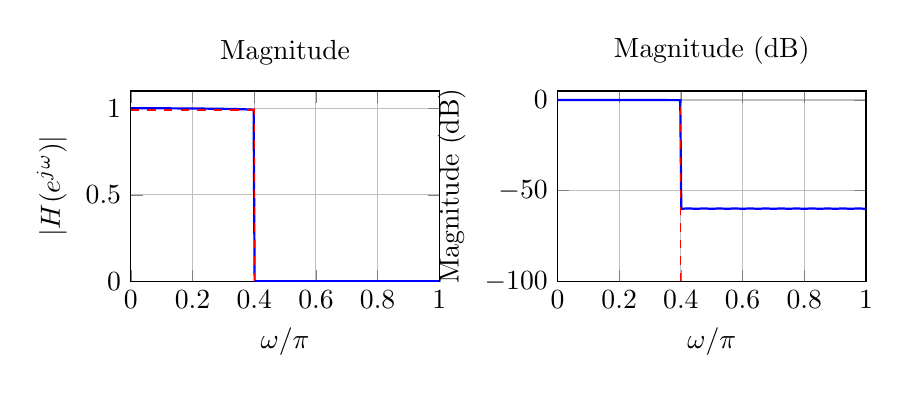
\begin{tikzpicture}
\begin{groupplot}[
    group style={
        group size=2 by 1,
        horizontal sep=1.5cm,
    },
    width=5.5cm,
    height=4cm,
]

% Linear magnitude
\nextgroupplot[
    xlabel={$\omega/\pi$},
    ylabel={$|H(e^{j\omega})|$},
    xmin=0, xmax=1,
    ymin=0, ymax=1.1,
    grid=major,
    title={Magnitude},
]
% Chebyshev Type II - monotonic passband, ripple in stopband
\addplot[blue, thick, domain=0:1, samples=300] {
  (x < 0.4) ? (0.99 + 0.01*(1 - (x/0.4)^2)^0.5) : 
  (0.001*(1 + 0.02*abs(sin(deg(8*3.14159*(x-0.6)/0.4)))))
};
\draw[red, dashed] (axis cs:0,0.99) -- (axis cs:0.4,0.99);
\draw[red, dashed] (axis cs:0. 4,0) -- (axis cs:0. 4,1);

% Log magnitude (dB)
\nextgroupplot[
    xlabel={$\omega/\pi$},
    ylabel={Magnitude (dB)},
    xmin=0, xmax=1,
    ymin=-100, ymax=5,
    grid=major,
    title={Magnitude (dB)},
]
\addplot[blue, thick, domain=0:1, samples=300] {
  (x < 0.4) ? (20*log10(0.99 + 0.01*(1 - (x/0.4)^2)^0.5)) : 
  (20*log10(0.001*(1 + 0.02*abs(sin(deg(8*3.14159*(x-0. 6)/0.4))))))
};
\draw[red, dashed] (axis cs:0. 4,-100) -- (axis cs:0.4,0);
\draw[blue, dashed] (axis cs:0.6,-60) -- (axis cs:1,-60);

\end{groupplot}
\end{tikzpicture}
\end{center}

\vspace{0.1cm}
\textbf{Characteristics:}
\begin{itemize}
  \item Monotonic in passband (smooth like Butterworth)
  \item Equiripple in stopband (oscillates around $\delta_s$)
  \item Stopband nulls from zeros on unit circle
\end{itemize}

\end{frame}

%--------------------------------------------------
\begin{frame}{Chebyshev Type II: Pole-Zero Plot}
\small

\textbf{Order 8 Chebyshev Type II Filter}

\vspace{0.2cm}
\begin{center}
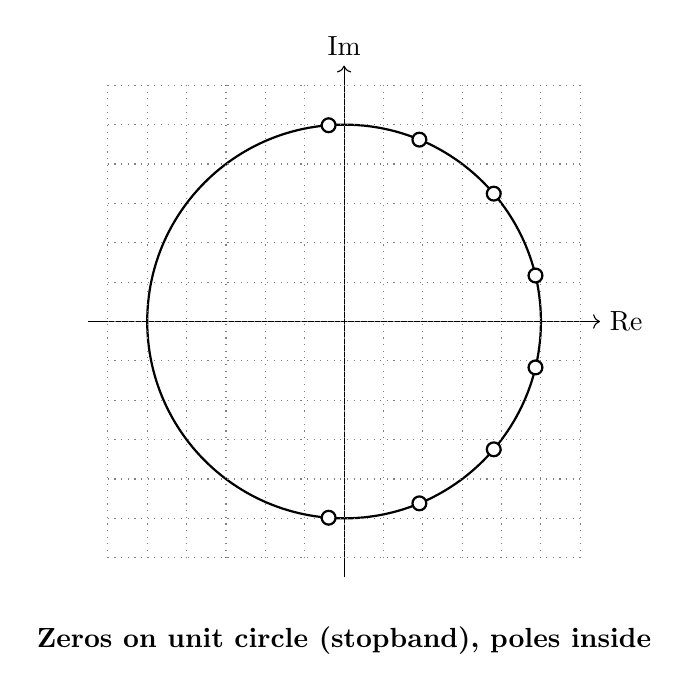
\begin{tikzpicture}[scale=2.5]
  % Unit circle
  \draw[thick] (0,0) circle (1);
  \draw[->] (-1.3,0) -- (1.3,0) node[right] {Re};
  \draw[->] (0,-1.3) -- (0,1.3) node[above] {Im};
  
  % Grid
  \draw[gray, dotted] (-1. 2,-1.2) grid[step=0.2] (1.2,1.2);
  
  % 8 zeros on unit circle in stopband (starting from 0. 6π)
  \foreach \i in {1,...,8} {
    \pgfmathsetmacro{\angle}{-108 + 216*(\i-0.5)/8}
    \node[circle, fill=white, draw=black, thick, minimum size=5pt, inner sep=0] at (\angle:1) {};
  }
  
  % Poles (8 poles inside unit circle)
  \foreach \i in {1,...,8} {
    \pgfmathsetmacro{\angle}{180 - 180*(\i-0.5)/8}
    \pgfmathsetmacro{\radiusx}{0. 65}
    \pgfmathsetmacro{\radiusy}{0.88}
    \pgfmathsetmacro{\xpos}{\radiusx*cos(\angle)}
    \pgfmathsetmacro{\ypos}{\radiusy*sin(\angle)}
    \node[mark=x, mark size=3pt, color=red] at (\xpos,\ypos) {};
  }
  
  \node[below] at (0,-1.5) {\textbf{Zeros on unit circle (stopband), poles inside}};
\end{tikzpicture}
\end{center}

\textbf{Key Features:}
\begin{itemize}
  \item 8 zeros distributed on unit circle in stopband region
  \item Zeros create nulls (complete attenuation) at specific frequencies
  \item More complex implementation than Type I
\end{itemize}

\end{frame}

%--------------------------------------------------
\section{Elliptic Filter}

\begin{frame}{Elliptic: Magnitude Response}
\small

\textbf{Order 6 Elliptic Filter (Optimal)}

\vspace{0.2cm}
\begin{center}
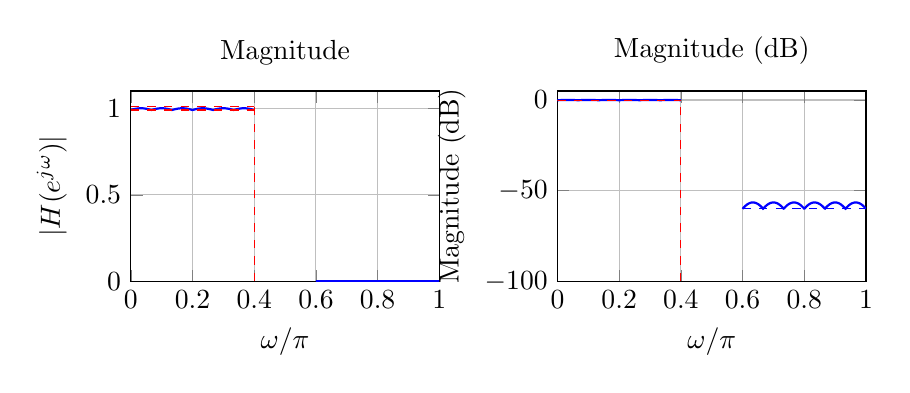
\begin{tikzpicture}
\begin{groupplot}[
    group style={
        group size=2 by 1,
        horizontal sep=1.5cm,
    },
    width=5.5cm,
    height=4cm,
]

% Linear magnitude
\nextgroupplot[
    xlabel={$\omega/\pi$},
    ylabel={$|H(e^{j\omega})|$},
    xmin=0, xmax=1,
    ymin=0, ymax=1.1,
    grid=major,
    title={Magnitude},
]
% Elliptic - ripple in both passband and stopband
\addplot[blue, thick, domain=0:0.4, samples=200] {0.99 + 0.01*abs(sin(deg(6*3.14159*x/0.4)))};
\addplot[blue, thick, domain=0.6:1, samples=200] {0.001*(1 + 0.5*abs(sin(deg(6*3.14159*(x-0.6)/0.4))))};
\draw[red, dashed] (axis cs:0,0.99) -- (axis cs:0.4,0.99);
\draw[red, dashed] (axis cs:0,1.01) -- (axis cs:0.4,1.01);
\draw[red, dashed] (axis cs:0. 4,0) -- (axis cs:0.4,1.01);

% Log magnitude (dB)
\nextgroupplot[
    xlabel={$\omega/\pi$},
    ylabel={Magnitude (dB)},
    xmin=0, xmax=1,
    ymin=-100, ymax=5,
    grid=major,
    title={Magnitude (dB)},
]
\addplot[blue, thick, domain=0:0.4, samples=200] {20*log10(0.99 + 0.01*abs(sin(deg(6*3.14159*x/0. 4))))};
\addplot[blue, thick, domain=0. 6:1, samples=200] {20*log10(0. 001*(1 + 0. 5*abs(sin(deg(6*3.14159*(x-0.6)/0.4)))))};
\draw[red, dashed] (axis cs:0,-0.087) -- (axis cs:0.4,-0.087);
\draw[red, dashed] (axis cs:0. 4,-100) -- (axis cs:0.4,0);
\draw[blue, dashed] (axis cs:0.6,-60) -- (axis cs:1,-60);

\end{groupplot}
\end{tikzpicture}
\end{center}

\vspace{0.1cm}
\textbf{Characteristics:}
\begin{itemize}
  \item Equiripple in \emph{both} passband and stopband
  \item Sharpest transition band (only 6th order!)
  \item Optimal filter (lowest order for given specs)
\end{itemize}

\end{frame}

%--------------------------------------------------
\begin{frame}{Elliptic: Pole-Zero Plot}
\small

\textbf{Order 6 Elliptic Filter}

\vspace{0.2cm}
\begin{center}
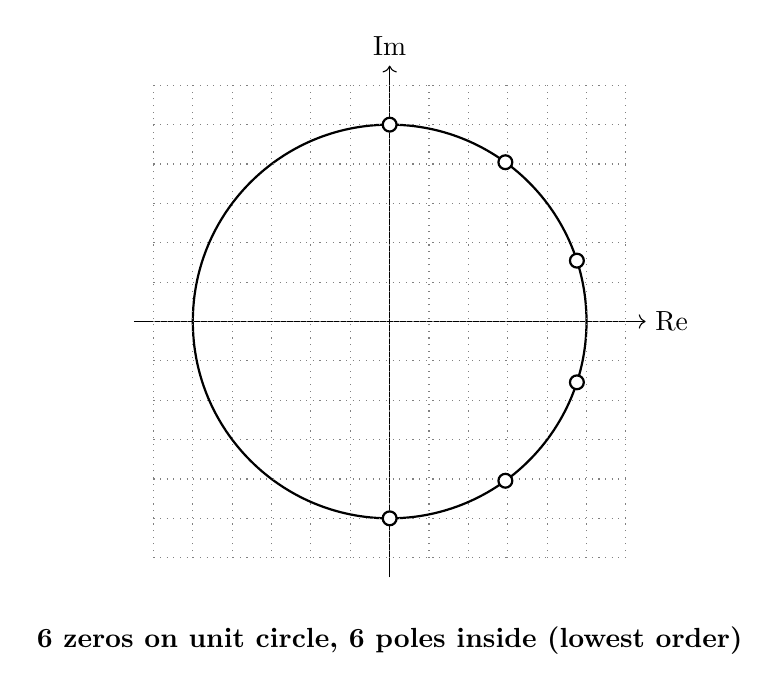
\begin{tikzpicture}[scale=2.5]
  % Unit circle
  \draw[thick] (0,0) circle (1);
  \draw[->] (-1.3,0) -- (1.3,0) node[right] {Re};
  \draw[->] (0,-1.3) -- (0,1.3) node[above] {Im};
  
  % Grid
  \draw[gray, dotted] (-1.2,-1.2) grid[step=0.2] (1.2,1.2);
  
  % 6 zeros on unit circle in stopband
  \foreach \i in {1,...,6} {
    \pgfmathsetmacro{\angle}{-108 + 216*(\i-0.5)/6}
    \node[circle, fill=white, draw=black, thick, minimum size=5pt, inner sep=0] at (\angle:1) {};
  }
  
  % 6 poles inside unit circle (ellipse)
  \foreach \i in {1,...,6} {
    \pgfmathsetmacro{\angle}{180 - 180*(\i-0.5)/6}
    \pgfmathsetmacro{\radiusx}{0.6}
    \pgfmathsetmacro{\radiusy}{0.85}
    \pgfmathsetmacro{\xpos}{\radiusx*cos(\angle)}
    \pgfmathsetmacro{\ypos}{\radiusy*sin(\angle)}
    \node[mark=x, mark size=3pt, color=red] at (\xpos,\ypos) {};
  }
  
  \node[below] at (0,-1.5) {\textbf{6 zeros on unit circle, 6 poles inside (lowest order)}};
\end{tikzpicture}
\end{center}

\textbf{Key Features:}
\begin{itemize}
  \item Only 6 poles and 6 zeros (vs.  14 for Butterworth!)
  \item Zeros on unit circle create stopband ripple
  \item Optimal pole-zero placement for minimum order
\end{itemize}

\end{frame}

%--------------------------------------------------
\section{Visual Comparison}

\begin{frame}{Side-by-Side Comparison: Magnitude}
\small

\begin{center}
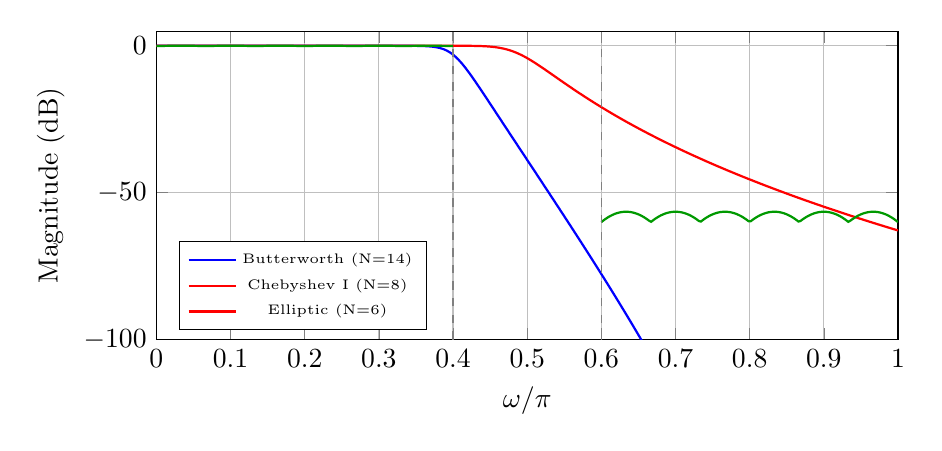
\begin{tikzpicture}
\begin{axis}[
    width=11cm,
    height=5. 5cm,
    xlabel={$\omega/\pi$},
    ylabel={Magnitude (dB)},
    xmin=0, xmax=1,
    ymin=-100, ymax=5,
    grid=major,
    legend pos=south west,
    legend style={font=\tiny},
]

% Butterworth N=14
\addplot[blue, thick, domain=0:1, samples=200] {20*log10(1/sqrt(1 + (tan(x*90)/tan(36))^28))};
\addlegendentry{Butterworth (N=14)}

% Chebyshev I N=8 (approximation)
\addplot[red, thick, domain=0:0.4, samples=150] {20*log10(1/(sqrt(1 + 0.01*0.01*(cos(8*acos(x/0.4)))^2)))};
\addplot[red, thick, domain=0.4:1, samples=150] {20*log10(1/(sqrt(1 + 0.01*0.01*(cosh(8*ln((x/0.4)+sqrt((x/0.4)^2-1))))^2)))};
\addlegendentry{Chebyshev I (N=8)}

% Elliptic N=6 (simplified)
\addplot[green! 60!black, thick, domain=0:0.4, samples=150] {20*log10(0.99 + 0.01*abs(sin(deg(6*3.14159*x/0.4))))};
\addplot[green!60!black, thick, domain=0.6:1, samples=150] {20*log10(0.001*(1 + 0.5*abs(sin(deg(6*3.14159*(x-0. 6)/0.4)))))};
\addlegendentry{Elliptic (N=6)}

% Spec lines
\draw[dashed, gray] (axis cs:0. 4,-100) -- (axis cs:0.4,5);
\draw[dashed, gray] (axis cs:0. 6,-100) -- (axis cs:0.6,5);

\end{axis}
\end{tikzpicture}
\end{center}

\textbf{Observations:}
\begin{itemize}
  \item Elliptic has sharpest transition (lowest order)
  \item Butterworth smoothest, but requires highest order
  \item All meet specifications, different trade-offs
\end{itemize}

\end{frame}

%--------------------------------------------------
\section{Conclusion}

\begin{frame}{Key Takeaways}
\small

\textbf{Visual Summary:}

\vspace{0.3cm}
\begin{center}
\small
\begin{tabular}{lccc}
\hline
\textbf{Type} & \textbf{Order} & \textbf{Passband} & \textbf{Stopband} \\
\hline
Butterworth & 14 & Monotonic & Monotonic \\
Chebyshev I & 8 & Equiripple & Monotonic \\
Chebyshev II & 8 & Monotonic & Equiripple \\
Elliptic & 6 & Equiripple & Equiripple \\
\hline
\end{tabular}
\end{center}

\vspace{0.3cm}
\textbf{Selection Guide:}
\begin{itemize}
  \item \textbf{Minimize order/cost? } $\rightarrow$ Elliptic
  \item \textbf{Smooth response?} $\rightarrow$ Butterworth
  \item \textbf{Balance efficiency \& simplicity?} $\rightarrow$ Chebyshev I
  \item \textbf{Smooth passband, lower order?} $\rightarrow$ Chebyshev II
\end{itemize}

\vspace{0.3cm}
\textbf{All zeros at $z=-1$:} Butterworth, Chebyshev I (simpler implementation)

\textbf{Zeros on unit circle:} Chebyshev II, Elliptic (stopband nulls)

\end{frame}





\end{document}

